\documentclass{article}
\usepackage[utf8]{inputenc}
\usepackage[a4paper, left=1cm, right=1cm, top=1cm, bottom=1cm]{geometry}
\usepackage{tikz}
\usepackage{hyperref}
\usetikzlibrary{positioning,shadings}
\usetikzlibrary{arrows}
\usetikzlibrary {shapes.geometric} 

\begin{document}
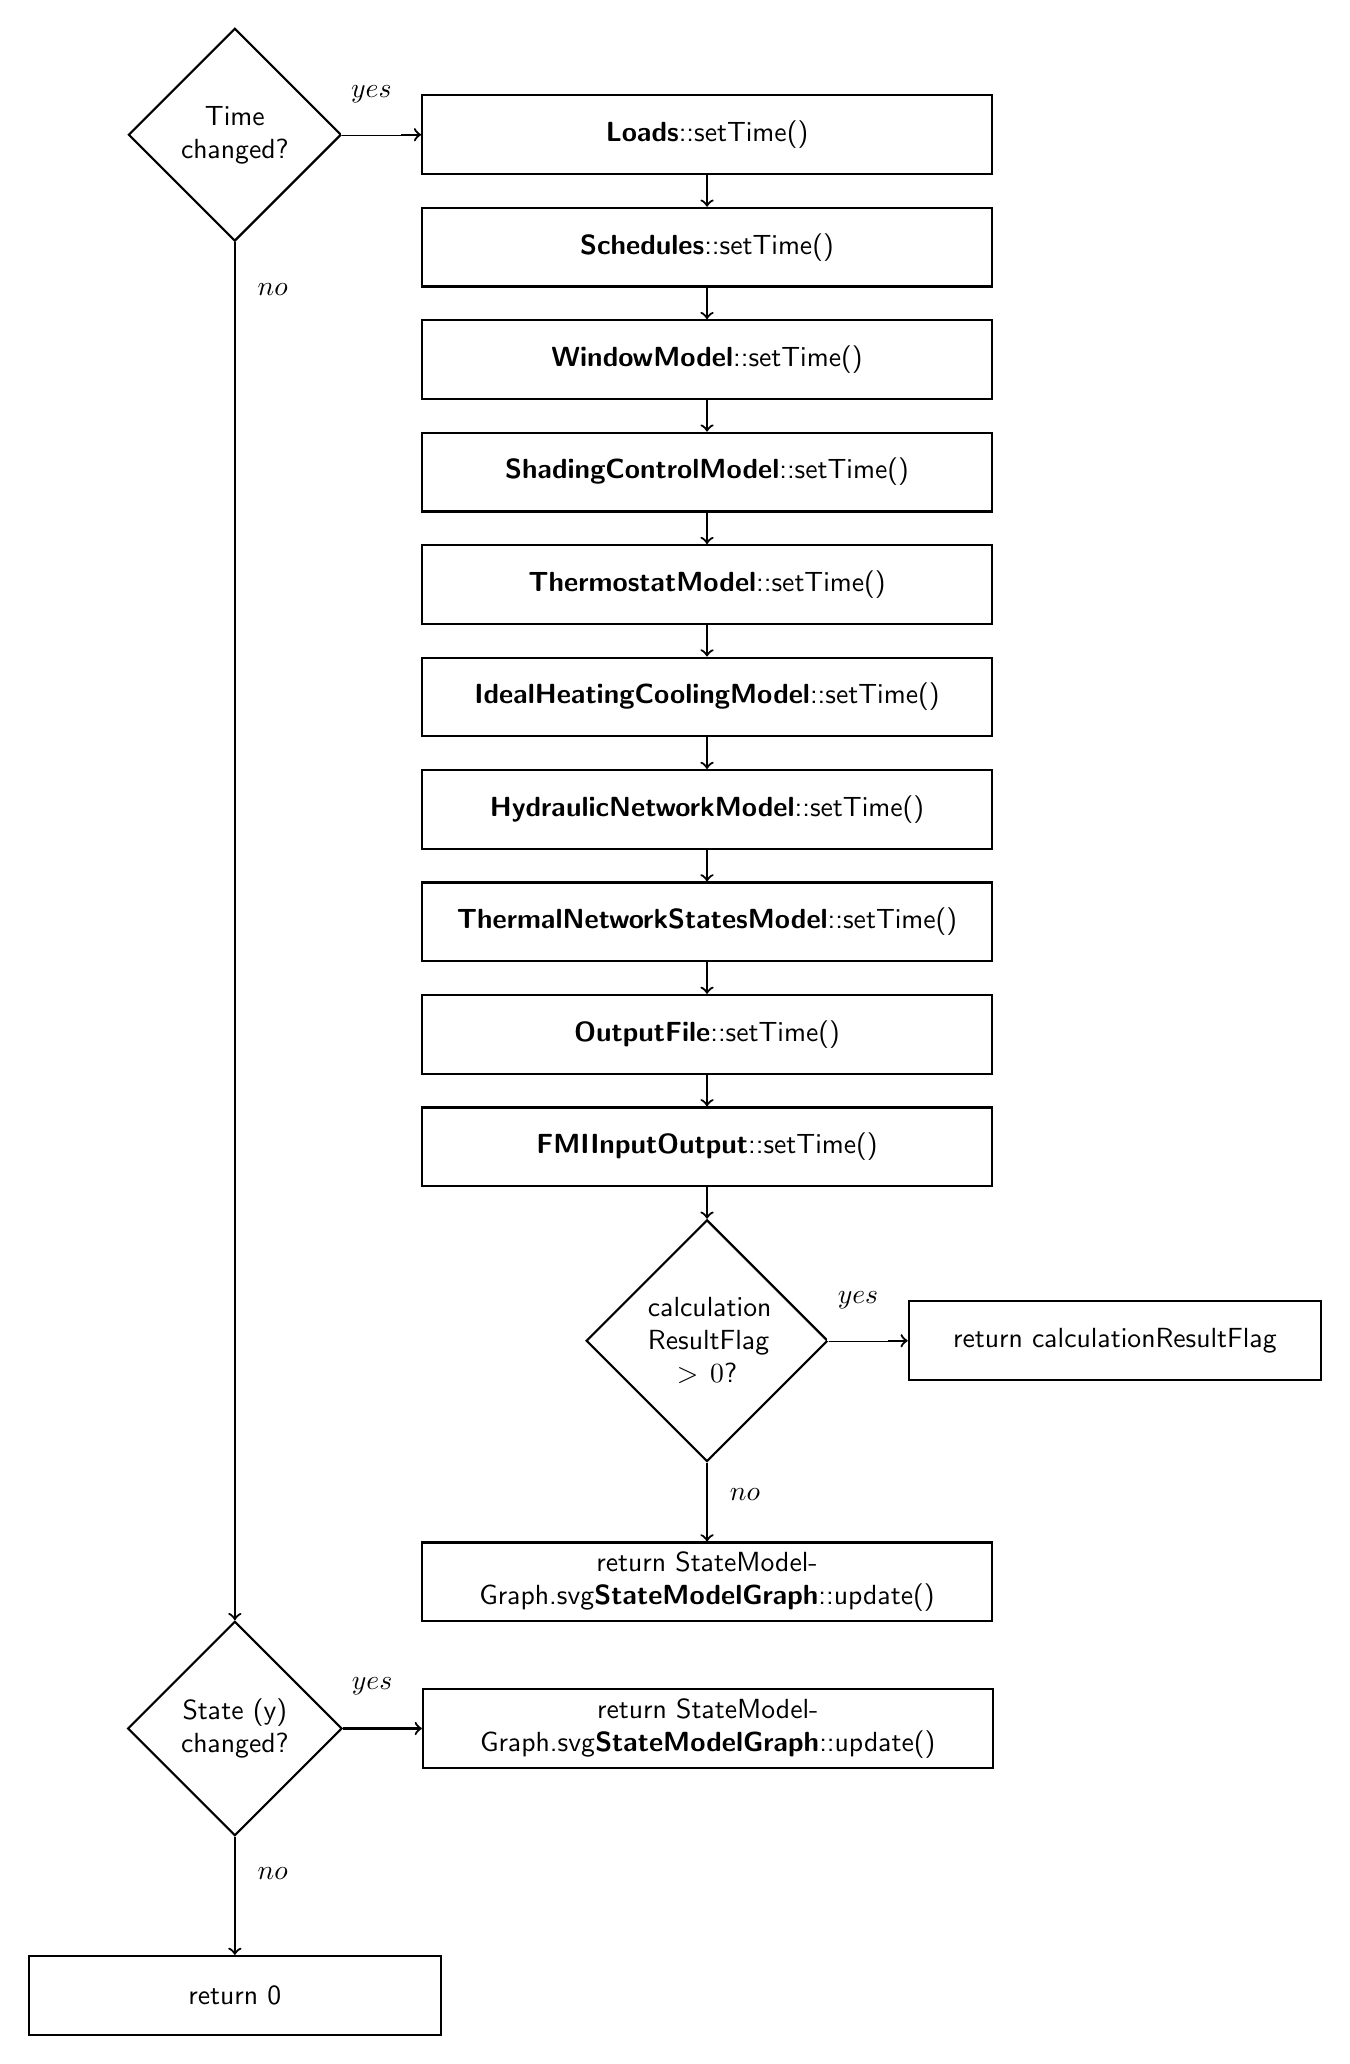
\begin{tikzpicture}[auto, node distance = 0.4cm, thick,
  every node/.style = {rectangle, font = \sffamily, draw=black,
    top color = white, bottom color = white,
    text width = 7cm, align = center, minimum height = 1cm}]
 
  \node (TimeDeps) [diamond, text width = 1.5cm]  {Time changed?};
  \node (Loads) [right = 1cm of TimeDeps]          {\textbf{Loads}::setTime()};
  \node (Sched) [below = of Loads]  {\textbf{Schedules}::setTime()};
  \node (Window) [below = of Sched]  {\textbf{WindowModel}::setTime()};
  \node (Shad) [below = of Window]  {\textbf{ShadingControlModel}::setTime()};
  \node (Therm) [below = of Shad]  {\textbf{ThermostatModel}::setTime()};
  \node (HeatCool) [below = of Therm]  {\textbf{IdealHeatingCoolingModel}::setTime()};
  \node (Network) [below = of HeatCool]  {\textbf{HydraulicNetworkModel}::setTime()};
  \node (ThermNet) [below = of Network]  {\textbf{ThermalNetworkStatesModel}::setTime()};
  \node (Output) [below = of ThermNet]  {\textbf{OutputFile}::setTime()};
  \node (FMI) [below = of Output]  {\textbf{FMIInputOutput}::setTime()};
  \node(calcRes) [diamond, text width = 1.5cm, below = of FMI] {calculation\\ResultFlag\\ $> 0$?};
  
  \node(Failure) [text width = 5cm, right = 1cm of calcRes] {return calculationResultFlag};

  \node (TimeStateGraph) [below = 1cm of calcRes]  {return \href{StateModelGraph.svg}{\textbf{StateModelGraph}}::update()};
  
  \node (StateDeps)[diamond, text width = 1.5cm, below = 17.5cm of TimeDeps]  {State (y) changed?};
  \node (StateGraph) [right = 1cm of StateDeps]  {return \href{StateModelGraph.svg}{\textbf{StateModelGraph}}::update()};

  \node (Success) [below = 1.5cm of StateDeps, text width = 5cm]  {return 0};
 
  \path[->]  
    (TimeDeps) edge[bend left=0] node[pos=0.35,above,draw=white,text width=0.5cm] {$yes$}  (Loads)
    (TimeDeps) edge[bend left=0] node[pos=0.03,right = 0.1cm,draw=white,text width=0.5cm] {$no$}  (StateDeps)
  
    (Loads) edge[bend left=0]  (Sched)
    (Sched) edge[bend left=0]   (Window)
    (Window) edge[bend left=0]  (Shad)
    (Shad) edge[bend left=0]   (Therm)
    (Therm) edge[bend left=0]   (HeatCool)
    (HeatCool) edge[bend left=0]   (Network)
    (Network) edge[bend left=0]   (ThermNet)
    (ThermNet) edge[bend left=0]  (Output)   
    (Output) edge[bend left=0]   (FMI)
    (FMI) edge[bend left=0]   (calcRes)

    (calcRes) edge[bend left=0]  node[pos=0.35,above,draw=white,text width=0.5cm] {$yes$}  (Failure)
    (calcRes) edge[bend left=0]   node[pos=0.4,right = 0.1cm,draw=white,text width=0.5cm] {$no$} (TimeStateGraph)
   
   
    (StateDeps) edge[bend left=0] node[pos=0.35,above = 0.02cm,draw=white,text width=0.5cm] {$yes$} (StateGraph)
    (StateDeps) edge[bend left=0] node[pos=0.3,right = 0.1cm,draw=white,text width=0.5cm] {$no$}  (Success);

\end{tikzpicture}
\end{document}